\appendix



\begin{appendices}
	\section{Phrases to Test K-Means}
	The phrases with which the K-Means algorithm was tested are shown below:
	\label{phrases}
\renewcommand\labelitemi{---}
	\begin{itemize}
\item 			 coronavirus hits remote utah
		\item scottish wind power success 
\item 		trump passes bill
		\item covid
		\item aboriginal peoples australia complain
		\item nikkei closes 90 points down
	\end{itemize}

	\section{K-Means Clustering k=3}
	\label{k3}
	\begin{figure}[H]
		\centering
		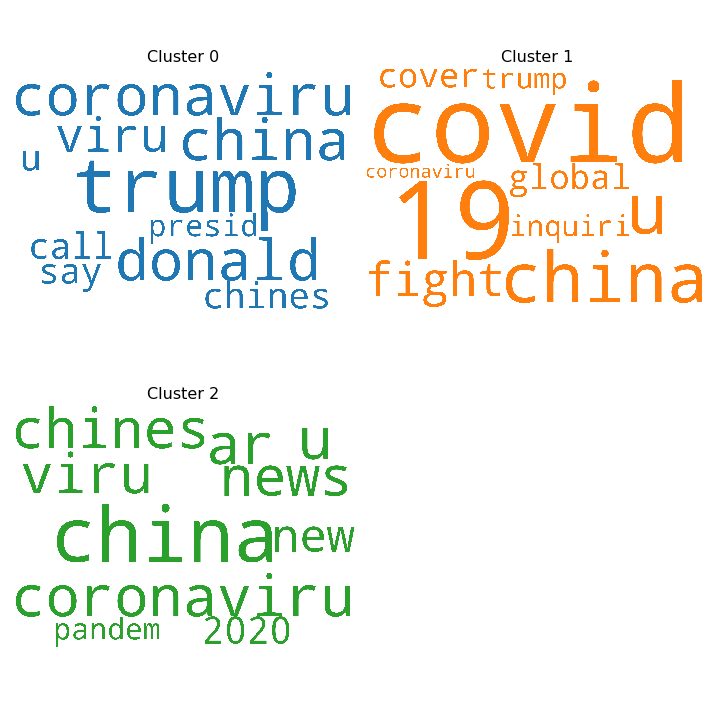
\includegraphics[width=0.8\textwidth]{images/kmeans_word_cloud_k=3.png}
		\caption{Word Cloud for k=3 clusters}
		\label{fig:wck3}
	\end{figure}
	
	\begin{figure}[H]
		\centering
		\subfloat[2D PCA k=3]{  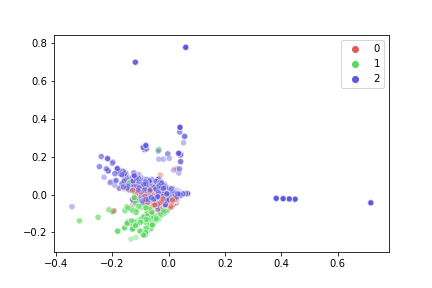
\includegraphics[width=0.45\textwidth]{images/kmeans_2d_pca_k=3.png}\label{fig:pca2k3}}
		\subfloat[3D PCA k=3]{  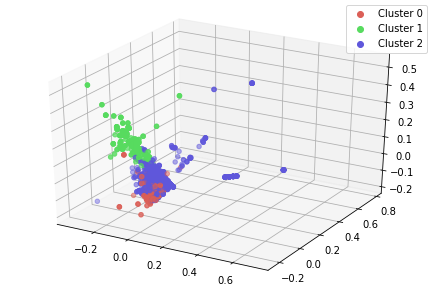
\includegraphics[width=0.45\textwidth]{images/kmeans_3d_pca_k=3.png}\label{fig:pca3k3}}\\
		\subfloat[2D T-SNE k=3]{  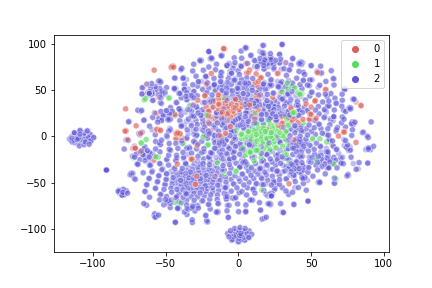
\includegraphics[width=0.45\textwidth]{images/kmeans_2d_tsne_k=3.png}\label{fig:ts2k3}}
		\subfloat[3D T-SNE k=3]{  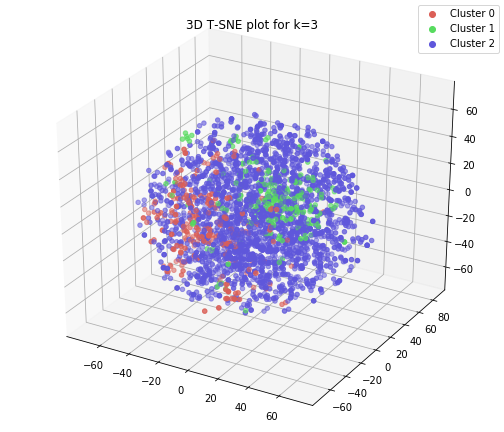
\includegraphics[width=0.45\textwidth]{images/kmeans_3d_tsne_k=3.png}\label{fig:ts3k3}}\\
		\caption{Decompositions of the clusters in 2 and 3 dimensions using PCA and T-SNE for k=3}
		\label{fig:k3pca}
	\end{figure}
	
	\begin{figure}[H]
		\centering
		\subfloat[Mahalanobis Distance]{  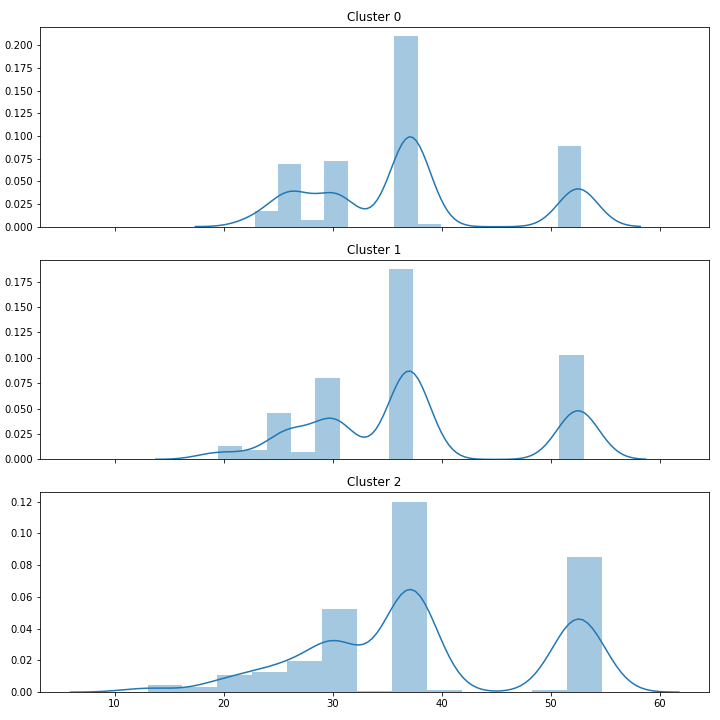
\includegraphics[width=0.45\textwidth]{images/kmeans_mahalanobis_distance_k=3.png}\label{fig:mhk3}}
		\subfloat[Euclidean Distances]{  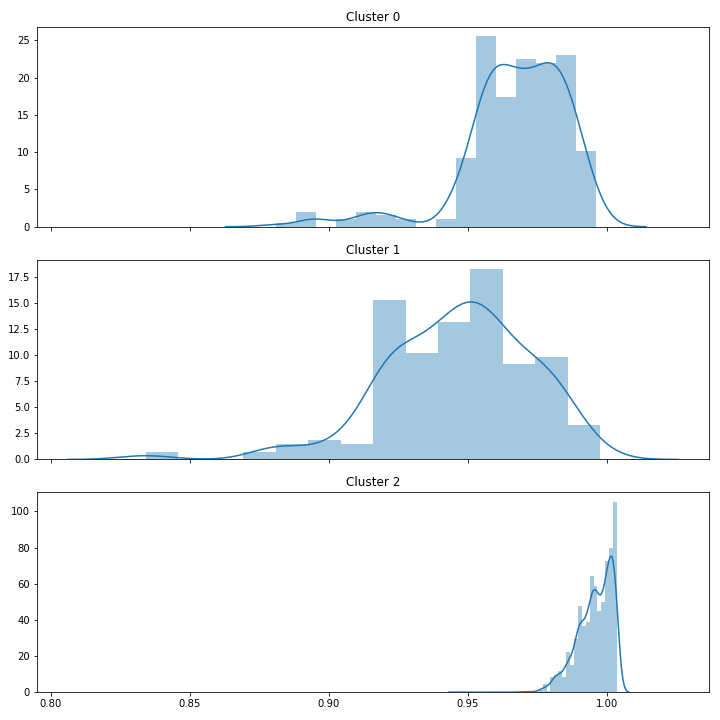
\includegraphics[width=0.45\textwidth]{images/kmeans_euclidean_distance_k=3.png}\label{fig:euk3}}\\
		
		\caption{Cluster Distances (Mahalanobis and Euclidean) for k=3 clusters}
		\label{fig:distk3}
	\end{figure}
	
	\begin{figure}[H]
		\centering
		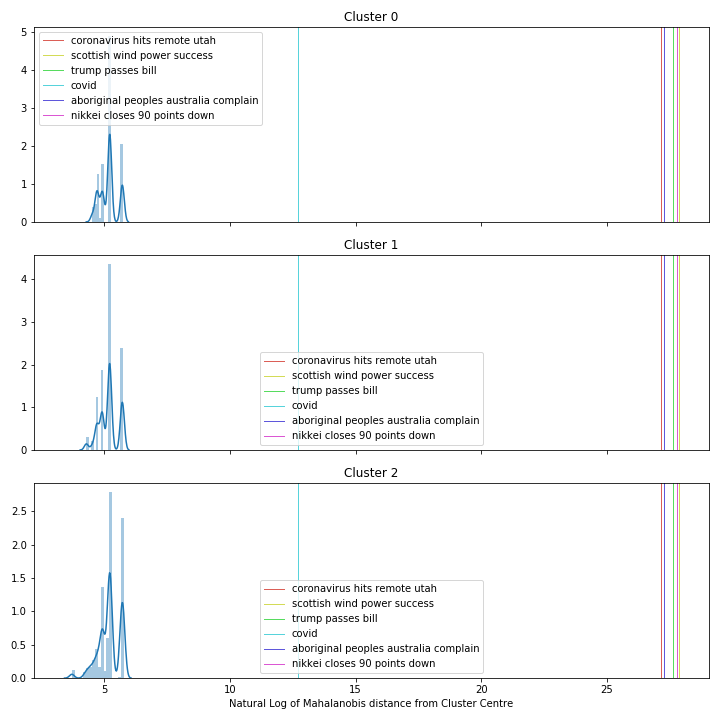
\includegraphics[width=0.8\textwidth]{images/words_kmeans_mahalanobis_distance_k=3.png}
		\caption{Log of Mahalanobis Distances for Clusters and Selected Phrases for k=3 clusters}
		\label{fig:wordsk3}
	\end{figure}
	\section{K-Means Clustering k=4}
	\label{k4}
	\begin{figure}[H]
		\centering
		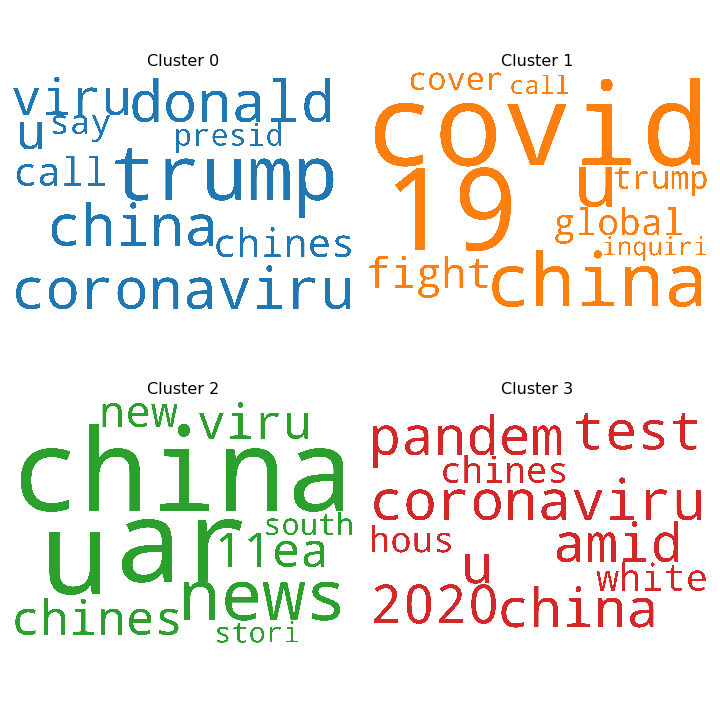
\includegraphics[width=0.8\textwidth]{images/kmeans_word_cloud_k=4.png}
		\caption{Word Cloud for k=4 clusters}
		\label{fig:wck4}
	\end{figure}
	
	
	\begin{figure}[H]
		\centering
		\subfloat[2D PCA k=4]{  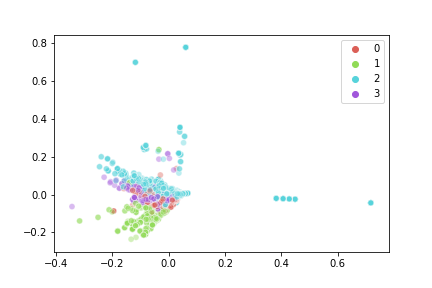
\includegraphics[width=0.45\textwidth]{images/kmeans_2d_pca_k=4.png}\label{fig:pca2k4}}
		\subfloat[3D PCA k=4]{  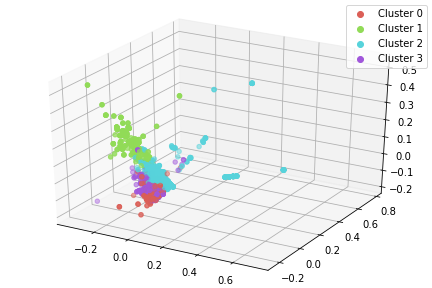
\includegraphics[width=0.45\textwidth]{images/kmeans_3d_pca_k=4.png}\label{fig:pca3k4}}\\
		\subfloat[2D T-SNE k=4]{  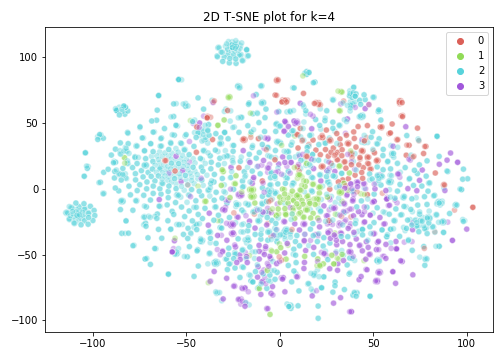
\includegraphics[width=0.45\textwidth]{images/kmeans_2d_tsne_k=4.png}\label{fig:ts2k4}}
		\subfloat[3D T-SNE k=4]{  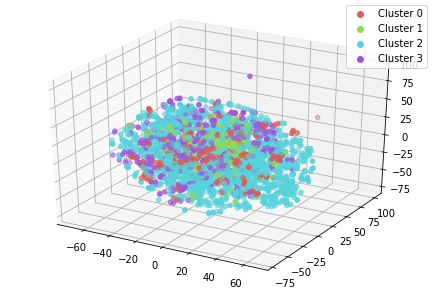
\includegraphics[width=0.45\textwidth]{images/kmeans_3d_tsne_k=4.png}\label{fig:ts3k4}}\\
		\caption{Decompositions of the clusters in 2 and 3 dimensions using PCA and T-SNE for k=4}
		\label{fig:k4pca}
	\end{figure}
	
	\begin{figure}[H]
		\centering
		\subfloat[Mahalanobis Distance]{  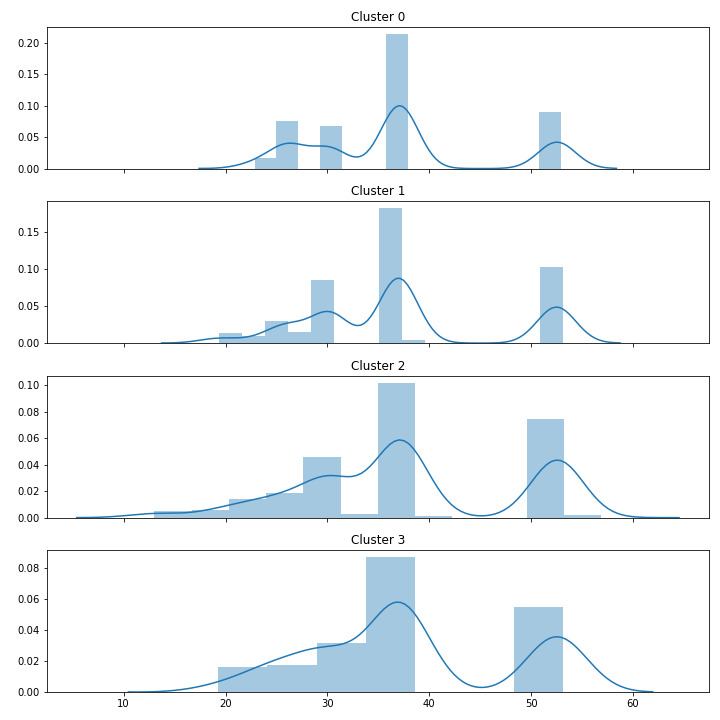
\includegraphics[width=0.45\textwidth]{images/kmeans_mahalanobis_distance_k=4.png}\label{fig:mhk4}}
		\subfloat[Euclidean Distances]{  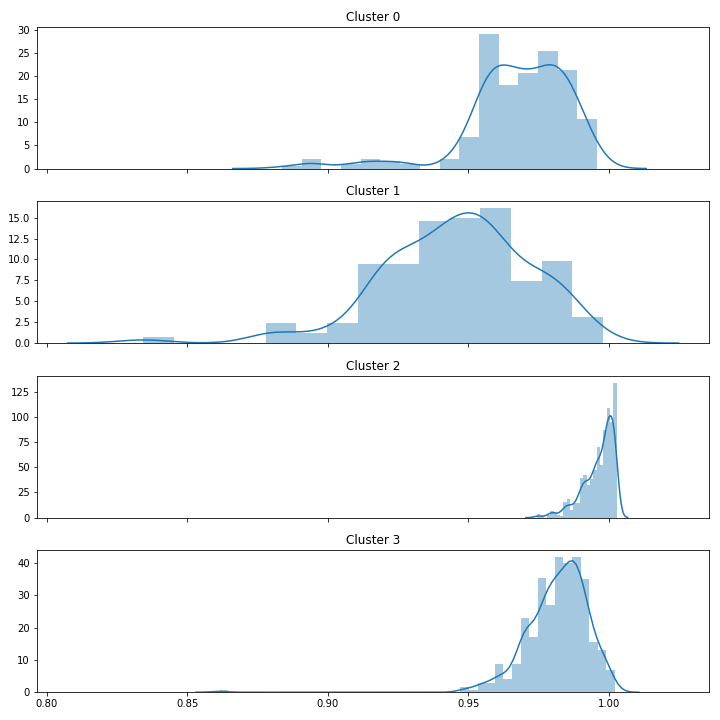
\includegraphics[width=0.45\textwidth]{images/kmeans_euclidean_distance_k=4.png}\label{fig:euk4}}\\
		
		\caption{Cluster Distances (Mahalanobis and Euclidean) for k=4 clusters}
		\label{fig:distk4}
	\end{figure}
	
	
	\begin{figure}[H]
		\centering
		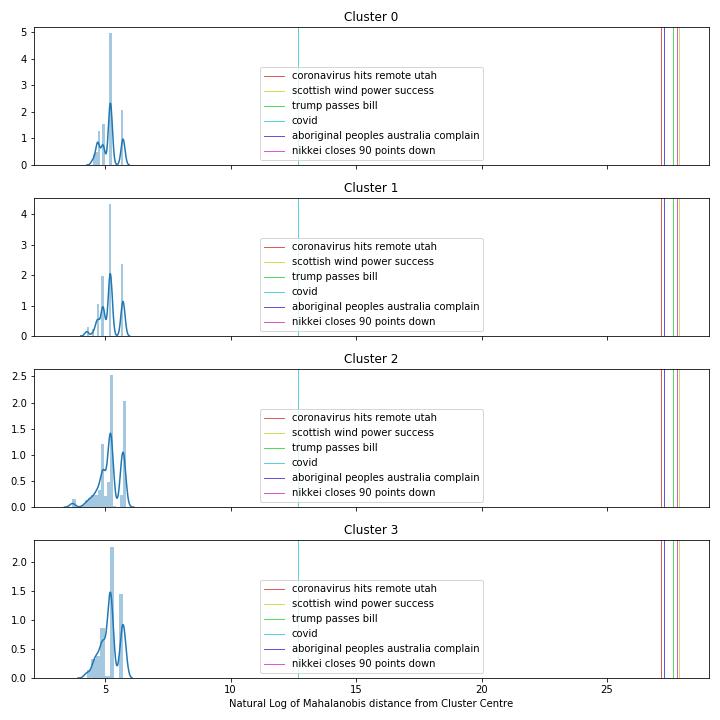
\includegraphics[width=0.8\textwidth]{images/words_kmeans_mahalanobis_distance_k=4.png}
		\caption{Log of Mahalanobis Distances for Clusters and Selected Phrases for k=4 clusters}
		\label{fig:wordsk4}
	\end{figure}
\end{appendices}

